\section{Die Regeln}
\label{Regeln}
Diese Arbeit beschäftigt sich nur mit der meist verbreiteten Art von Sudokus. Dieses Sudoku spielt man auf einem Spielfeld der Größe 9x9. Das beudeutet, dass jede Seite des Sudokus 9 Felder lang ist. Das Spielfeld ist in 9 Blöcke der Größe 3x3 unterteilt. Es hat ausserdem 9 Zeilen und 9 Spalten. Insgesamt besteht das Sudokus also aus 81 Felder. In das Sudoku werden im Spielverlauf Ziffern eingetragen, so, dass am Ende des Spiels jedes Feld gefüllt ist. Dabei gilt ein Sudoku als gelöst, wenn in jeder Zeile, in jeder Spalte und in jedem Block die Ziffern 1 bis 9 jeweils einmal vorkommen. Das ist die einzige Regel des Sudokuspiels.\\

\begin{figure}[h]
\begin{center}
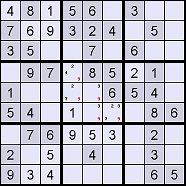
\includegraphics{./img/sudoku.jpg}
\caption{Sudoku}
\end{center}
\end{figure}

\noindent In \textbf{Abbildung 2.1} sieht man ein unfertiges Sudoku. Im mittleren Block kann man sehen, dass in einigen Feldern mehrere kleine Zahlen eingetragen sind. Diese dienen als Gedankenstütze des Spielers und helfen ihm beim Finden komplexer Muster, die für einige Lösungstechniken benötigt werden. Das notieren dieser Zahlen ist allerdings keine Pflicht.\\
Wichtig ist bei Sudokus, dass ein Sudoku nur als solches gilt, wenn es genau eine Lösung hat. Es sind keine Anordnungen der Zahlen erlaubt, die mehrere Lösungen zulassen, oder die schon von Anfang an im Widerspruch zur Sudokuregel stehen oder unvermeidbar zu einem Widerspruch führen.\\